\documentclass[10.5pt,compress]{beamer}
\usepackage[utf8]{inputenc}

\newcounter{saveenumi}
\newcommand{\seti}{\setcounter{saveenumi}{\value{enumi}}}
\newcommand{\conti}{\setcounter{enumi}{\value{saveenumi}}}

%\usepackage{amsmath}
\usepackage{amsmath}
\usepackage[ruled,longend]{algorithm2e}
%\usepackage[ruled,longend]{algpseudocode}
%\usepackage{algorithm}
\usepackage{pifont}
\usepackage{amsmath,amssymb}
\usepackage{geometry}
\usepackage{xparse}
\usepackage{multirow}
\usepackage{tikz-qtree-compat}
\tikzset{every tree node/.style={baseline=(left.base),
level distance=2em, sibling distance=4em, align=center,
parent anchor=south, child anchor=north, anchor=north}, sibling distance=15pt}
 \usetikzlibrary{positioning}
 \usetikzlibrary{decorations}
\usepackage{tikz}
\usepgflibrary{arrows}% for more options on arrows
\newcommand{\argmin}{\arg\!\min}
\usepackage[absolute,overlay]{textpos}
\usepackage{graphicx} 
\usepackage{eurosym}
\usepackage{xcolor}
%\usetheme{AnnArbor}
%\usetheme{Antibes}
%\usetheme{Bergen}
%\usetheme{Berkeley}
%\usetheme{Berlin}
%\usetheme{Boadilla}
%\usetheme{boxes}
%\usetheme{CambridgeUS}
%\usetheme{Copenhagen}
%\usetheme{Darmstadt}
%\usetheme{default}
\usetheme{Dresden}
\usepackage{media9}
%\usetheme{Frankfurt}
%\usetheme{Goettingen}
%\usetheme{Hannover}
%\usetheme{Ilmenau}
%\usetheme{JuanLesPins}
%\usetheme{Luebeck}
%\usetheme{Madrid}
%\usetheme{Malmoe}
%\usetheme{Marburg}
\usepackage{mathrsfs}
%\usetheme{Montpellier}
%\usecolortheme{crane}
%\usecolortheme{albatross}
%\usecolortheme{beaver}
%\usecolortheme{beetle}
%\usecolortheme{crane}
%\usecolortheme{dolphin}
%\usecolortheme{dove}
%\usecolortheme{fly}
%\usecolortheme{lily}
%\usecolortheme{orchid}
\usecolortheme{rose}
%\usecolortheme{seagull}
%\usecolortheme{seahorse}
%\usecolortheme{whale}
%\usecolortheme{wolverine}
%\usetheme{Pittsburgh}
%\usetheme{Rochester}
%\usetheme{Singapore}
%\usetheme{Szeged}
%\usetheme{Warsaw}
\usepackage[english]{babel}
\usepackage{listings}
\usepackage{url}
\usepackage{hyperref}
%\usepackage{enumitem}
%\usepackage{etoolbox}
%\makeatletter
%\patchcmd{\beamer@continueautobreak}{\frametitle}{\beamer@gobbleoptional}{}{\errmessage{failed to patch}}
%\patchcmd{\beamer@continueautobreak}{\framesubtitle}{\beamer@gobbleoptional}{}{\errmessage{failed to patch}}
%\makeatother
\newtheorem{mydef}{Definition}
\newtheorem{myprop}{Proposition}
\newtheorem{myexample}{Example}
\setbeamertemplate{theorems}[numbered]
%\newcommand*{\underarrow}[1]{\ensuremath{\underset{\downarrow}{#1}}}
%\NewDocumentCommand{\Underarrow}{O{} O{\downarrow} m}{%
%  \underset{\makebox[0pt]{\begin{tabular}{@{}@{}}\ensuremath{#2}\\[0pt]\end{tabular}}}{#1}}
\def\blegend#1#2{\underset{\underset{\scriptstyle\text{#2}}{\scriptstyle\updownarrow}}{#1}}

\useoutertheme{infolines}
\title[Confidential Transactions - Initial Overview]{Confidential Transactions - Initial Overview}
\usepackage{remreset}
\mode<presentation>


%\usecolortheme{whale}
%\usecolortheme{orchid}
\usecolortheme[named=orange]{structure} 
\useinnertheme{circles}
\useoutertheme{miniframes}

\makeatletter
\@removefromreset{subsection}{section}
\makeatother
%\setcounter{subsection}{1}
\usepackage{etoolbox}
\makeatletter
\patchcmd{\slideentry}{\ifnum#2>0}{\ifnum2>0}{}{\@error{unable to patch}}% replace %the subsection number test with a test that always returns true
\makeatother

%\titlegraphic{\hspace*{7.5cm}~%
%   \includegraphics[width=1.8cm]{Logo_Politecnico_Milano}
%}


\author[Alessandro Miola]{
Alessandro Miola}
% - Give the names in the same order as the appear in the paper.
% - Use the \inst{?} command only if the authors have different
%   affiliation.

\institute[] % (optional, but mostly needed)
{}

% - Use the \inst command only if there are several affiliations.
% - Keep it simple, no one is interested in your street address.

\date[September 2018]{September, 2018}

\begin{document}
\renewcommand*{\inserttotalframenumber}{\pageref{lastframe}}

\begin{frame}
  \titlepage
\end{frame}



\subsection{Building a Range Proof - Borromean ring signatures' role}
\begin{frame}{Building a RP - I$^{st}$ issue: how Borromean ring signatures get into}
    \underline{Recall}: RP is an additional piece of data needed to prove the committed amount lies in a range of positive values (the amount must neither be negative, nor exceed the field order), without disclosing the committed amount itself (Zero Knowledge RP).
    \begin{itemize}
        \item With the tools presented, it's now possible to prove it.
        \item The prominent role played by Borromean ring signatures will be soon evident. It was somehow previewed before, slide ~\ref{ring-sing-on-PC}.
    \end{itemize}
\end{frame}

\begin{frame}[allowframebreaks]
    \begin{alertblock}{Example} 
        Consider again the tx presented before, slide ~\ref{tx}.\\
        Let's say that Alice creates a \underline{single} output (for simplicity), of value 2,010 BTC.
    \end{alertblock}
    \begin{enumerate}
        \item Need to define what an appropriate range would be.
        \begin{itemize}
            \item As amounts in Bitcoin transactions are encoded in 32-bit integer data, the definition of the range is straightforward.\\
            \underline{Minimum amount}: \textbf{0} BTC\\
            \underline{Maximum amount}: \textbf{42.94967295} BTC \\(i.e. 4294967295 satoshis = $2^{32}-1$ satoshis, maximum amount storable in a 32-bit integer data).
            \item This also explains the anticipation at slide ~\ref{range}, \textbf{range =} $\boldsymbol{[0,2^{32})}$.
        \end{itemize}
        \framebreak
        \item Create a Pedersen commitment to the tx value (v = 201000000 satoshis).
        \begin{equation*}
            C = rG + vH 
        \end{equation*}
        \item Construct an associated Range Proof.
        \begin{enumerate}
            \item Write the output amount in its \textit{binary} expansion (although an optimization considering base-4 encoding will come later).
            \begin{equation*}
                v = v_0\cdot2^0 + v_1\cdot2^1 + v_2\cdot2^2 + \dots + v_{31}\cdot2^{31}
            \end{equation*}
            \underline{Decimal amount}: 201000000 satoshis.\\
            \underline{Binary amount}: 00001011111110110000010001000000 satoshis.
            \framebreak
            \item \textbf{Ring-sign} (with a Borromean-style ring signature) \textbf{over each digit}.
            %% proper explanation on how to do it when considering the base-4 optimization, as it is the one really used. --> anzi NO, la faccio da entrambe le parti..
            \begin{itemize}
                \item \textbf{1 ring per digit}, \textbf{2 verification pubkeys per ring} (a pubkey committing to 0, the other committing to 1).\\
                $\Rightarrow$ 32 rings, 2 pubkeys each corresponding to digit values (0,1).
                \item \textbf{For each digit create a Pedersen commitment}, making sure the sum of the commitments corresponds to C. 
                \begin{equation*}
                    C_i = r_iG + v_i2^iH
                \end{equation*}
                which is either a commitment to \textbf{0} or to $\boldsymbol{2^i}$, without revealing which.\\
                %% aim that is accomplished by means of the following step, thus by providing a ring signature.
                \underline{Example}: fifth digit from the left (value = 1) in the binary representation $\rightarrow$ amount = $2^{27} = 134217728$\\
                $\Rightarrow$ Construct the following commitment:
                %% Obviously secret blinding factor r_4 needed here (together with all the others 31 blindind factors), ma trattiamo dopo il setting dei blinding factors. 
                \begin{equation*}
                    C_4 = r_4G + 134217728H
                \end{equation*}
                \framebreak
                %% con pubkey si intende commitment pubkey, i.e. Pedersen commitment ovviamente
                \item \textbf{Arrange for one pubkey per digit to be \textit{``signable-for"}}.
                That is, provide a Borromean ring signature over the ring:\\
                \begin{equation*}
                    \{\boldsymbol{r_iG + v_i2^iH}, \boldsymbol{r_iG + v_i2^iH - 2^iH}\}
                \end{equation*}
                $\Rightarrow$ if $v_i \notin$ \{0,1\}, then neither of the keys in the ring will be a commitment to 0, thus preventing the ring to be signable for (see even slide ~\ref{0_1_commit}).\\
                \underline{Example}: given the digit considered before, construct the following set of pubkeys:
                \footnote{\tiny{$0H = 0\cdot2^{27}H$}}
                \begin{align*}
                    C_{40} &= C_4 - 0H\\ 
                    C_{41} &= C_4 - 134217728H
                \end{align*}
                Then perform a Borromean ring signature and particularly perform a \textbf{real} signature for $C_{41} = \underbrace{C_4}_{r_4G + 134217728H} - 134217728H = r_4G$\\
                (for which $r_4$ is known).
                \framebreak 
                \item \textbf{Signature size}: the final RP of the value v is:\\
                %% per quanto riguarda le commitment pubkey (i.e. i Pedersen commitments), che non fanno parte della Borromean ring signature, si pubblicano i soli commitment "signable for", i commitments chosen for each of the rings
                \begin{equation*}
                    \boldsymbol{RP_v = (C_0, \dots, C_{31}, \underbrace{e_0, s_0, \bar{s}_0, s_1, \bar{s}_1, \dots, s_{31}, \bar{s}_{31}}_{Borromean})}.
                \end{equation*}
                Thus, in total: 1 e-value + 32*2 s-values + 32 commitment pubkeys (about 3KB of data).\\ % considering 97 32-bytes number which is however a simplification because in reality pubkeys are 33 bytes long + some other adjustment.
                It would be possible however to save something in terms of space usage by means of a different encoding for the committed value.
            \end{itemize}
            \item Consider to use a different encoding for the committed value.\\ 32 bit numbers:
            % Considering non-powers of 2 is messier in programming terms.
            \begin{itemize}
                \item base \textbf{2} $\rightarrow$ 1 bit per digit: 
                \begin{cases} 0 \quad $\leftrightarrow$ & \mbox{0 in bit} \\ 1 \quad $\leftrightarrow$ & \mbox{1 in bit} \end{cases}
                \item base \textbf{4} $\rightarrow$ 2 bits per digit:
                \begin{cases} 0 \quad $\leftrightarrow$ & \mbox{00 in bits} \\ 1 \quad $\leftrightarrow$ & \mbox{01 in bits} \\ 
                2 \quad $\leftrightarrow$ & \mbox{10 in bits} \\ 3 \quad $\leftrightarrow$ & \mbox{11 in bits}\\ \end{cases}
                \framebreak
                \item base \textbf{8} $\rightarrow$ 3 bits per digit:
                \begin{cases} 0 \quad $\leftrightarrow$ & \mbox{000 in bits} \\ 1 \quad $\leftrightarrow$ & \mbox{001 in bits} \\ \vdots \\
                6 \quad $\leftrightarrow$ & \mbox{110 in bits} \\ 7 \quad $\leftrightarrow$ & \mbox{111 in bits}\\ \end{cases}
                \item Given y is the number of bits-per-digit, the total number of pubkeys + s-values is given by:
                \begin{equation*}
                    \boxed{N(y) = \frac{32}{y} \cdot (1+2^y)}
                \end{equation*}
                \end{itemize}
                \begin{minipage}{.40\textwidth}
                \centering
                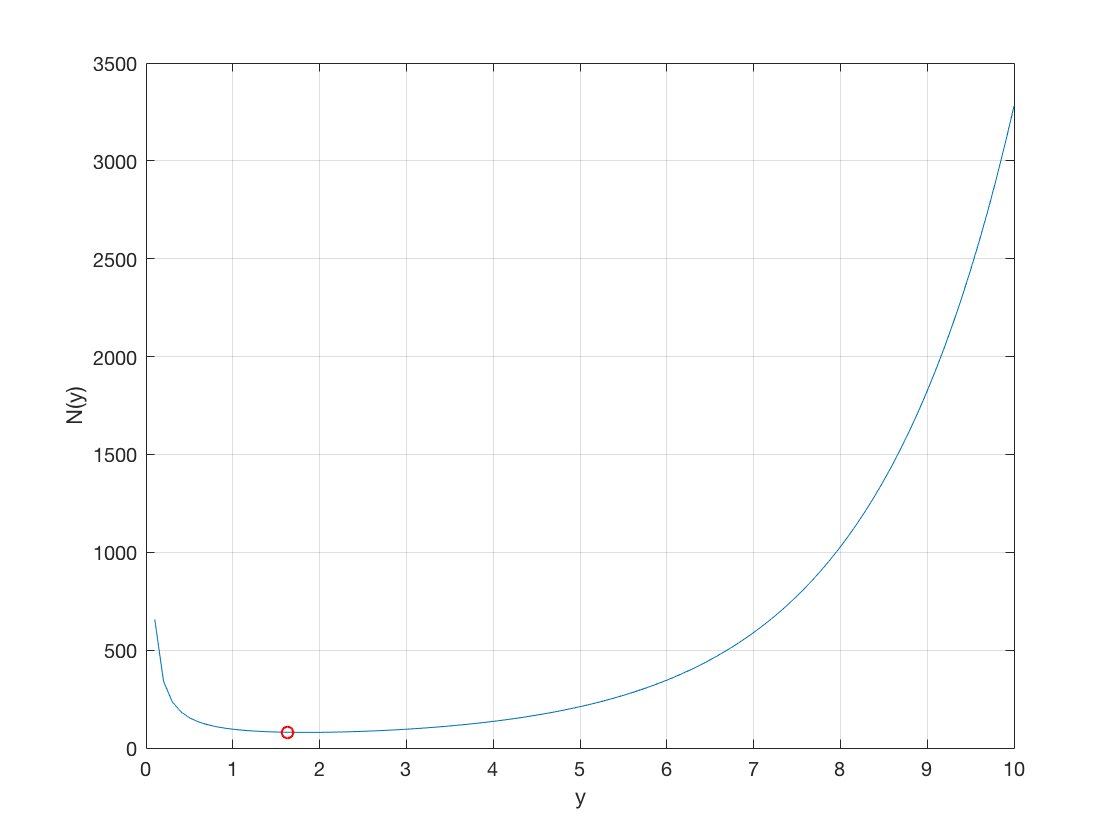
\includegraphics[,     width=.85\textwidth]{N_y.png}
                \end{minipage}%
                \begin{minipage}{.60\textwidth}
                \begin{itemize}
                    \item It takes the minimum around y=2 \\(2 bits per digit $\rightarrow$ base 4).
                    \item Amounts are represented via a\\ \textbf{base-4} encoding (i.e. rings of size 4)\\ as this minimizes the number of\\ commitments sent.
                \end{itemize}
                \end{minipage}%
            \framebreak
            \item Write the output amount in its \textit{base-4} expansion.
            \begin{equation*}
                v = v_0\cdot4^0 + v_1\cdot4^1 + v_2\cdot4^2 + \dots + v_{15}\cdot4^{15}
            \end{equation*}
            \underline{Decimal amount}: 201000000 satoshis.\\
            \underline{Base-4 amount}: 0023332300101000 satoshis.
            \item \textbf{Ring-sign} (with a Borromean-style ring signature) \textbf{over each digit}.
            \begin{itemize}
                \item Exactly like before. 1 ring per digit, 4 verification pubkeys per ring.
                \item Create a Pedersen commitment for each digit, making sure the sum of the commitments corresponds to C. 
                \begin{equation*}
                    C_i = r_iG + v_i4^iH
                \end{equation*}
                \underline{Example}: third digit from the left (value = 2) in the base-4 representation $\rightarrow$ amount = $2\cdot4^{13} = 134217728$\\
                $\Rightarrow$ Construct the following commitment:
                %% Obviously secret blinding factor r_2 needed here (together with all the others 15 blindind factors), ma trattiamo dopo il setting dei blinding factors. 
                \begin{equation*}
                    C_2 = r_2G + 134217728H
                \end{equation*}
            \framebreak
            \item Provide a Borromean ring signature over the ring:\\
            \begin{equation*}
            \{\boldsymbol{r_iG + v_i4^iH}, \boldsymbol{r_iG + v_i4^iH - 4^iH}\}
            \end{equation*}
            \underline{Example}: given the digit considered before, construct the following set of pubkeys:
            \begin{align*}
                    C_{20} &= C_2 - 0H\\ 
                    C_{21} &= C_2 - 67108864H\\
                    C_{22} &= C_2 - 134217728H\\
                    C_{23} &= C_2 - 201326592H
            \end{align*}
            Then perform a Borromean ring signature and particularly perform a \textbf{real} signature for $C_{22} = \underbrace{C_2}_{r_2G + 134217728H} - 134217728H = r_2G$\\
            (for which $r_2$ is known).
            %% collegamento con slide 31, posso firmare solo con un punto che sia multiplo esatto di G (necessary to have v=0).
            \item \textbf{Signature size}: 1 e-value + 16*4 s-values + 16 commitment pubkeys, which is about 2560 bytes (less than it was before).
            %% 16*5 = 80 32-byte strings
            \end{itemize}
        \end{enumerate}
    \end{enumerate}
\end{frame}

\subsection{Building a Range Proof - sender/receiver communication}
\begin{frame}{Building a RP - II$^{nd}$ issue: details of ECDH Key Exchange}
    \begin{alertblock}{Remark} 
        What is left out is what concerns sender/receiver communication about:
        \begin{itemize}
            \item setting of the \textbf{blinding factors}
            \item transmission of the \textbf{committed amount value}.
            %i blinding factors, come si vedrà tra pochissimo, sono settati dal sender, generati in modo deterministico (via scanning key) e pertanto riproducibili dal receiver as well semplicemente. il receiver runs the procedure on its own per recuperarli. 
            % vale anche per gli amount, sono XORati e il receiver li recupera facendo XOR a sua volta..
        \end{itemize}
    \end{alertblock}
    \underline{Recall}:
    \begin{itemize}
        \item From the point of view of the network, RPs just represent a proof that the amounts committed in a tx are valid, \underline{but} amounts (together with blinding factors) stay secret and only known to participants in the tx.
        %% "proof that the amounts committed in a tx are valid" --> e questo grazie alle (Borromean) ring signatures.
        \item As partly previewed (slide ~\ref{ECDH_No_interact} ff.), for security as well as efficiency issues, it is required for the transfer not to be interactive (no receiver's involvement). %% and the solution is ECDH
        % ff. è il corrispondente italiano di ss. (i.e. e pagine seguenti)
        \underline{Moreover}, it would be nice to have a \textbf{space-saving solution} to embed the secret information in the tx without leaking it.
        %%% and this is a great achievement in this RP construction!!!!
    \end{itemize}
\end{frame}

\begin{frame}
    % questa freccia verso il basso per ricollegarmi subito al l'"it would be nice .." della slide precedente lasciato aperto...
    \begin{center}
        $\Downarrow$
    \end{center}
    %It turns out that 
    The ultimate Range Proof's construction (at least the one involving Borromean ring signatures) enables the possibility to transfer safely tx value \& blinding factors:
    % con ultimate intendo di questa sezione
    \begin{itemize}
        \item w/ \textbf{no interactivity}
        %% no interaction in advance with the receiver
        \item \textbf{w/o adding more data in the tx} rather than commitments and RP.\\
        $\Rightarrow$ \textit{Amounts} are embedded in RP w/o taking up more space.\\
        $\Rightarrow$ \textit{Blinding factors} are part of a deterministic generation process; set by the sender and reproducible by sender and receiver only. %% rapida anticipazione del fatto che amounts sono embeddati nei RP senza che occupino ulteriore spazio, i blinding factors sono parte di un processo di generazione deterministica riproducibile dal receiver only (PERCHE QUESTI CONDIVIDE LA SCANNING KEY COL SENDER).
    \end{itemize}
    In addition to this, it even enables the possibility to \textbf{transfer arbitrary user-selected data} (always embedded in RP, no more space needed). 
    % user = sender!
    % no more space needed rather than RP itself
\end{frame}

% gia si è detto a grandi linee che la maniera in cui vengono trasmessi i blinding factors e l'amount è attraverso un'"istanza" di ECDH. In realtà questa definisce la shared key che viene poi utilizzata dalle parti (sender e receiver) per runnare RFC6979 e generare le stesse qtà.  
\begin{frame}{ECDH role}
    To point out something already anticipated,
    \begin{itemize}
        \item each party in a CT has a separate ephemeral pubkey for ECDH purpose only (\textbf{scanning key}),
        % called scanning key because it enables scanning/reading of the private transaction information.
        \item an instance of ECDH serves to define a \textbf{shared key}.
        \begin{itemize}
            \item The scheme is the standard one, seen at slide ~\ref{ECDH}.
            \item a, b play the role of ECDH ephemeral private keys.
        \end{itemize}
    \end{itemize}
    \underline{Then}, 
    \begin{itemize}
        \item this shared key is exploited by both tx sender and receiver to deduce the same blinding factors (and not only them).
    \end{itemize}
\end{frame}

\begin{frame}{}
    \textbf{\underline{Scanning key}}:
    %% CT addresses = addresses used by Elements alpha sidechain
    \begin{itemize}
        \item CT addresses have a different format wrt standard Bitcoin addresses (they are longer than the latter).
        \item Each CT address embeds a scanning (pub)key for ECDH.
        \item Format:
        \end{itemize}
        \begin{center}
            \textbf{base58check}(\textbf{$<$scanning key version byte$>$ $<$standard address version byte$>$ $<$scanning key$>$ $<$standard address data bytes$>$})
        \end{center}
        % Observe that being the private key associated to the shared key deriving from the ECDH istance separated from the private key for spending, the parties could potentially share the private key for ECDH and thus exposing the values and the msgs embedded in the txs. (Selective Transparency). For instance, it could be useful if they want to share a whole set of txs.
\end{frame}

\begin{frame}{RFC6979 deterministic generation}
    \begin{itemize}
        \item \textbf{Blinding factors}
        \item \textbf{Random s-values} needed for Borromean ring signatures
    \end{itemize}
    are both part of a deterministic generation process via RFC6979, with the \textbf{shared key} derived from ECDH used to \textit{seed} a RFC6979 prng.\\ \ \\
    Making this process \textit{deterministic}, provides some sort of advantages (besides the ones already discussed).\\
    %% quelli already discussed sarebbero quelli relativi all'assenza di interattività nel trasferimento (due to ECDH).
\end{frame}

\begin{frame}
    Especially important among these advantanges is the possibility to distinguish \textit{where randomness resides} \footnote{\tiny{The focus here is on fake signatures generation.}} and exploit this feature accordingly:
    \begin{itemize}
        % con RFC6979, per quanto riguarda le signature values e.g., si costruiscono solo le FAKE signatures e runnando la medesima procedura sia sender che receiver sanno dove stia tutta la randomness e possono sfruttare ciò ai propri (differenti) scopi..
        \item (for the sender) possibility to \textbf{send data} over the predetermined and forged signature values:
        \begin{itemize}
            \item send a specific information that needs transmission, the \textbf{committed tx output amount} % which is embedded into one of those fake signatures (usually the last one, if not forged)
            \item send other private messages to the designated tx receiver.
        \end{itemize}
        % "rewind the proof" proprio by knowing where randomness goes into 
        \item (for the receiver) possibility to \textbf{``rewind" the proof}, which implies:
        \begin{itemize}
            \item generating the same blinding factors of the sender
            \item reading out the tx output amount
            \item extract further messages the sender could have sent.
        \end{itemize}  
    \end{itemize}
\end{frame}

% Partire con dettagli, blinding factors setting, fake sig ecc, come da foglio 
\begin{frame}[allowframebreaks]
    \begin{enumerate}
        \item \textbf{Blinding factors' setting}
        % RFC6979 HMAC procedure used, which is the same procedure for generating pseudo random numbers (nonces and more) to be used in ECDSA signatures. Idea: create an instance of HMAC, w/ the privkey as source of entropy and the hash of the msg as the nonce. The pseudo random number is created from the output of this instance. Start w/ a seed value (generally the concatenation of private key and hashed msg H(m), vedi pag 14 documento RFC6979 tools.ietf.org) and hash "repeatedly". The process can be repeated by taking each output as input of the HMAC process, as many times as necessary.
        \begin{itemize}
            \item The 32-byte shared key derived from ECDH is used as first seed to a RFC6979 prng.
            \item Then, each output is used as next seed.
            \item Blinding factors $r_0, r_1, \dots, r_{15}$ are generated (although $r_{15}$ e.g. is chosen by difference so as to match the sum of blinding factors from inputs).
            % il fatto che lo faccia anche il receiver specificarlo dopo, nella proof rewind
        \end{itemize}
        \item \textbf{Forged signatures \& nonces' generation}\\
        \underline{Recall}: $\frac{3}{4}$ of the 64 s-values needed to construct the Borromean ring signature are forged, but need to be indistinguishable from random.
        \begin{itemize}
            % direi che semplicemtente si continuerà usando l'ultimo blinding factor ottenuto attraverso la RFC6979 procedure come primo input per generare il primo s-value falso, o qualcosa di simile..
            \item The RFC6979 prng is used to generate these \textbf{fake signature values}.
            % con RFC6979 HMAC procedure si generano random values per OGNUNO dei 64 s-values nel ring, ma per le 16 firme REALI questi random values sono usati come nonces
        \end{itemize}
        Moreover, even for what concerns the remaining $\frac{1}{4}$ of the signatures (the real ones), generation of random values is needed.
        \begin{itemize}
            \item The RFC6979 prng is used to generate the \textbf{nonces}.
            % direi non distinti dai forged s-values (sono entrambi 32-bytes random numbers), sono sempre parte del processo di generazione descritto prima. Poi laddove le signature debbano essere reali, saranno usati come nonces piuttosto che come s-values.
        \end{itemize}
        \framebreak
        \item \textbf{Committed tx amount's transmission}
        \begin{itemize}
            \item \underline{Idea}: embed the tx amount somewhere in the construction without letting it occupy more space. %rather than commitments and RP size.
            \item \underline{Solution}: embed it into \underline{one} of the forged signatures (usually the last one, unless it is a real one) by \textbf{XOR}ing \footnote{\tiny{XOR: bit-wise addition mod 2 (w/o carry). Properties:\\ A $\oplus$ 0 = A; \quad A $\oplus$ A = 0; \quad (A $\oplus$ B) $\oplus$ C = A $\oplus$ (B $\oplus$ C); \quad (B $\oplus$ A) $\oplus$ A = B $\oplus$ 0 = B.}} ($\oplus$) it \textbf{with the forged s-value for that signature}.
            \begin{itemize}
                \item XOR preserves the entropy of the original pseudo-random s-value. % the result stays totally random
                \item The amount is encoded with particular formatting details.
            \end{itemize}
        \end{itemize}
        \begin{enumerate}
            \item \textbf{Sender \& receiver's viewpoint}:\\
            Dealing with \underline{forged signatures only} (and consequently forged s-values only), let's consider:
            \begin{itemize}
                \item $\boldsymbol{s_{COMMON}}$: s-value deterministically generated from RFC6979 procedure. %and reproducible by both sender and receiver.
                \item $\boldsymbol{s_{PUBLISH}}$: s-value actually published by the sender in RP construction.
            \end{itemize}
            \framebreak
            \underline{Sender}:\\
            \begin{equation*}
                \fbox{s_{PUBLISH} = s_{COMMON} \oplus amount}
            \end{equation*}
            \underline{Receiver}:
            \begin{equation*}
                \fbox{s_{COMMON} \oplus s_{PUBLISH} = s_{COMMON} \oplus s_{COMMON} \oplus amount = amount}
            \end{equation*}
            Thus, the receiver, looking at the last (in general) signature and computing $s_{COMMON} \oplus s_{PUBLISH}$ sees:
            \begin{itemize}
                \item \underline{the amount} if the last signature is the one that has been tampered with the amount
                \item \underline{0} if the last signature hasn't been tampered with the amount, while still being forged.
            \end{itemize}
            \framebreak
            \item \textbf{Output amount (8-bytes value) encoding}:\\
            Consider again the example run in the previous subsection:\\
            \underline{Decimal amount}: 201000000 satoshis\\
            \underline{Hex amount (8 bytes) + single bytes decimal conversion}\footnote{\tiny{Necessary because XOR acts on single bytes. The idea is: XOR with single bytes decimal-converted number, pass to hexadecimal and then come back to decimal. It is built in such a way that the concatenation of bytes resulting from the XORing forms the hexadecimal number corresponding to the amount (in base 10).}}:
            % cioè è costruito in modo tale che i singoli bytes risultanti dall'XORing formino il numero esadecimale che corrisponde all'amount in base decimale.
            \begin{equation*}
            %\blegend{f(x)}{Integrand}
                \blegend{00}{0}\blegend{00}{0}\blegend{00}{0}\blegend{00}{0}\blegend{0B}{11}\blegend{FB}{251}\blegend{04}{4}\blegend{40}{64} 
            \end{equation*}
            %% recall: è possibile esprimere un byte con esattamente due cifre esadecimali.
            \item \textbf{XOR the amount in 3 separate places into the last of the 64 signatures} (if forged)
            \begin{itemize}
                \item XORing in 3 separate fixed places into the last 32 byte value.
                %\item This is done to make the probability of occurrence of such a repeating pattern null in case
                \item Need to XOR the number ``128" with the $I^{st}$ byte of the s-value of the considered signature to avoid an issue that would occurr with null amounts.
                \item If the s-value into the last signature is not forged, do the same on the last but one.\\ \underline{Indeed}, real signatures mustn't be tampered with and the reason why is clear: the real s-value is \textit{necessary} to close the ring and validate the signature.
            \end{itemize}
        \end{enumerate}
        \framebreak
        \textbf{\underline{Remark}} \ding{172}: the amount takes 32 bytes only, all the rest (less the space corresponding to the real s-values) is left for the transmission of generic data (about the 80\% of the proof's size).\\ % less the space corresponding to the real s-values which is however replaced by the space for nonces that seems to be tamperable with (CAPISCI MEGLIO QUESTO, anche se, sì, non dovrebbe influenzare)...
        %% According to ciò, in teoria, 2016/2560 = 78.75% of the proof's size could be used for priv msgs communication.
        \textbf{\underline{Remark}} \ding{173}: 
        \begin{itemize}
            \item \textbf{if} no forged signature has been XORed in,
        \end{itemize}
        the tx receiver could potentially deduce the amount in another way. He could look at all the s-values and check which ones can be generated via RFC6979 procedure, the other being necessarily real ones. Knowing which are real, he can deduce the amount accordingly.
        However,
        \begin{itemize}
            \item this is not the best solution as it would preclude sending other messages.
        \end{itemize}
        \textbf{\underline{Remark}} \ding{174}: in the end, the forged s-values (at least some of these, 1 minimum) published as part of the RP are the result of a XORing.
        %% CONTROLLA, pensaci ancora, ma direi di si, non cambia nulla...
        % Direi che non cambia nulla proprio in virtu del fatto che XORing preserva l'entropia degli s-values originari 
        \framebreak
        \item \textbf{Other user-defined data's transmission}
        \begin{itemize}
            \item Basically, it works the same as before.
            \item The only difference is that some user-defined data rather than the tx amount is XORed in with the random s-values.
        \end{itemize}
        \item \textbf{Proof's ``rewind" by the receiver}\\
        Given the shared key, the receiver can run the same RFC6979 procedure of the sender and deduce:
        \begin{itemize}
            \item same blinding factors
            \item same forged s-values.
        \end{itemize}
        Then,
        \begin{itemize}
            \item he can perform the XOR operation as said before.
        \end{itemize}
        \framebreak
        According to our example, if the considered signature is effectively the one tampered with the amount, the result of the XOR should be something like this (with the repetitions occurring in positions 9-16, 17-24, 25-32 e.g.):
        \end{enumerate}
        \begin{equation*} 
            \fbox{128,0,0,0,0,0,0,0,\underline{0,0,0,0,11,251,4,64},\underline{0,0,0,0,11,251,4,64},\underline{0,0,0,0,11,251,4,64}}            
        \end{equation*}
        % as already described
        The receiver would then:
        \begin{itemize}
            \item Convert each byte in its hexadecimal representation.
            \item Convert the whole hexadecimal number in base 10.
        \end{itemize}
\end{frame}

\subsection{Building a Range Proof - fee handling}
\begin{frame}{Building a RP - III$^{rd}$ issue: explicit fees}
    \begin{itemize}
        \item In a standard Bitcoin transaction the fee is \textit{implicit}, what comes out from the difference between input and output values.
        \item In CT, amounts are not published to the network $\rightarrow$ the fee amount \textbf{f} is published \textbf{explicitely} as it cannot be deduced implicitely as before.
        \begin{itemize}
            \item Published as a plaintext, 4-byte amount after the inputs and before the outputs.
        \end{itemize}
        \item Consequences on the commitment scheme:
        \begin{itemize}
            \item Construct a Pedersen commitment for the fee amount. %% da parte del transaction creator
            \item The necessity to keep fee amount explicit (which opposes to the Pedersen commitment's aim to obscure tx amount) makes it necessary for fees to be paid ``\textbf{unmasked}", just as \textbf{fH} rather than rG + fH. %% unmasked or unblinded
            \item Thus, it is built with blinding factor $\boldsymbol{r_f = 0}$.
        \end{itemize}
        \item The network just checks that $\sum_{i}C_i^{inp} - \sum_{i}C_i^{out} - fH = 0$.
    \end{itemize}
\end{frame}

\section{Schematic of a CT}
\begin{frame}{}
    \begin{figure}
        \centering
        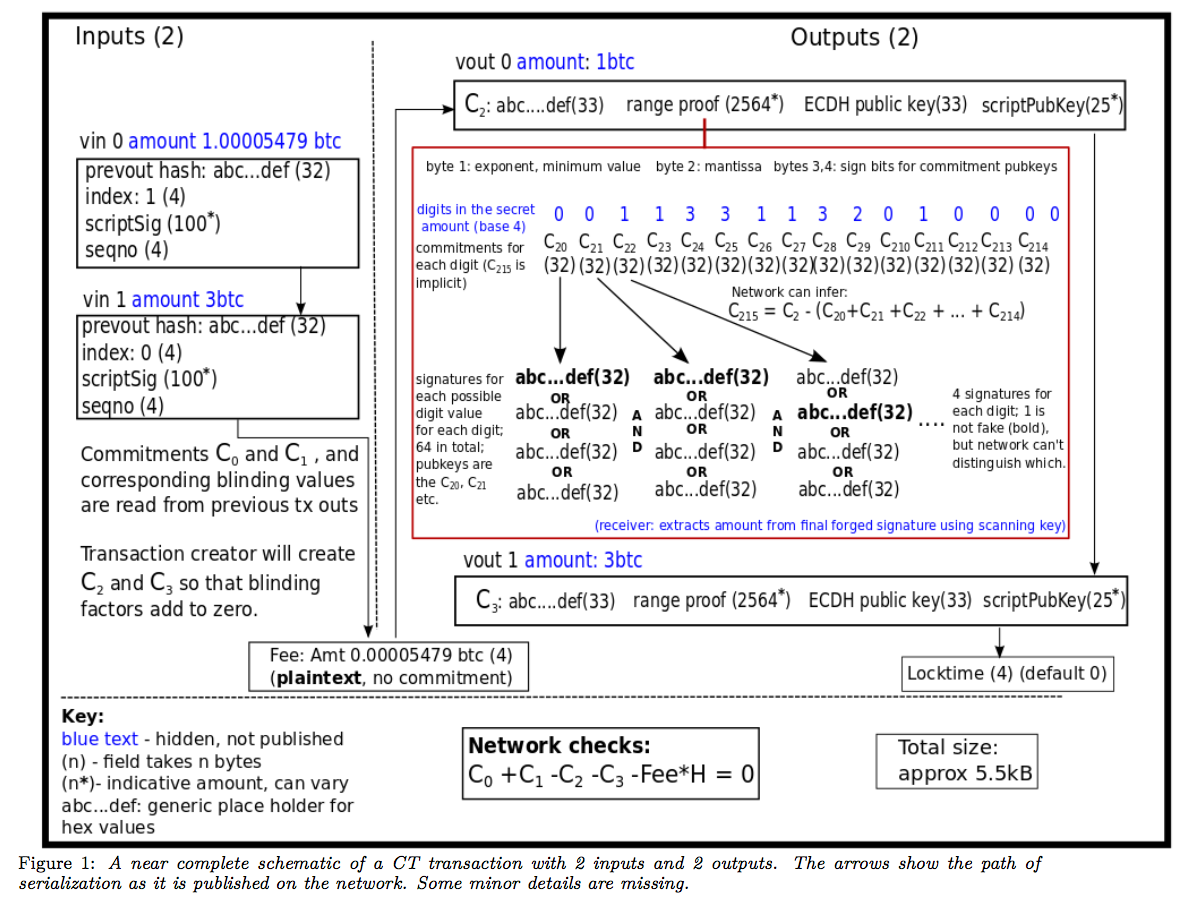
\includegraphics[scale = 0.475]{schema_tx.png}
        \tiny{\caption{\tiny{figure from ``An investigation into Confidential Transactions" - A. Gibson} }}
        %\label{fig:my_label}
    \end{figure}
\end{frame}

\section{Bibliography}
\begin{frame}{References}
   \begin{thebibliography}{triangle}
    \bibitem{}{\url{https://people.xiph.org/~greg/confidential_values.txt}}
    \bibitem{}{\url{https://github.com/AdamISZ/ConfidentialTransactionsDoc}}
    \bibitem{}{\url{https://github.com/Blockstream/borromean_paper/raw/master/borromean_draft_0.01_8c3f9e7.pdf}}
    \bibitem{}{Slides from - Bulletproofs: Short Proofs for Confidential Transactions and More}
    \newblock{B. Bünz, J. Bootle, D. Boneh, A. Poelstra, P. Wuille and G. Maxwell}
    \newblock{\url{https://crypto.stanford.edu/~buenz/publications/}}
    \bibitem{}{\url{https://bitcointalk.org/index.php?topic=1085273.40}}
    \bibitem{}{\url{https://github.com/AdamISZ/bulletproofs-poc}}
    \end{thebibliography}
\end{frame}

\begin{frame}
    \begin{thebibliography}{triangle}
    \bibitem{}{\url{http://diyhpl.us/wiki/transcripts/gmaxwell-confidential-transactions/}}
    \bibitem{}{\url{https://ledgerjournal.org/ojs/index.php/ledger/article/viewFile/34/61}}
    \bibitem{}{\url{http://cryptoservices.github.io/cryptography/2017/07/21/Sigs.html}}
    \bibitem{}{\url{https://moderncrypto.org/mail-archive/curves/2015/000534.html}}
    \bibitem{}{\url{https://bitcointalk.org/index.php?topic=285142.40}}
    \bibitem{}{\url{https://tools.ietf.org/html/rfc6979#section-3.2}}
    \bibitem{}{\url{https://bitcoin.stackexchange.com/questions/48064/sending-confidential-transaction-amount-to-the-receiver}}
    \item MANY MORE MISSING.....
    \end{thebibliography}
\end{frame}



\end{document}

